%% ============================================================
%%  RISC-V OoO CPU --- 答辩 Beamer 幻灯片
%%  编译命令: xelatex main.tex  (运行两次以生成正确页码)
%% ============================================================
\documentclass[aspectratio=169,xcolor={dvipsnames,svgnames},10pt]{beamer}

%% ─── 中文支持 ────────────────────────────────────────────────
\usepackage[UTF8]{ctex}

%% ─── 基础宏包 ────────────────────────────────────────────────
\usepackage{tikz}
\usetikzlibrary{arrows.meta,shapes.geometric,positioning,
                fit,backgrounds,calc,decorations.pathreplacing}
\usepackage{booktabs}
\usepackage{multirow}
\usepackage{array}
\usepackage{colortbl}
\usepackage{listings}
\usepackage{amsmath}

%% ─── 颜色定义 ────────────────────────────────────────────────
\definecolor{PrimaryBlue}  {RGB}{25,118,210}
\definecolor{DeepBlue}     {RGB}{13, 71,161}
\definecolor{LightBlue}    {RGB}{144,202,249}
\definecolor{PaleBg}       {RGB}{227,242,253}
\definecolor{AccentOrange} {RGB}{245,124,  0}
\definecolor{AccentGreen}  {RGB}{ 46,125, 50}
\definecolor{AccentRed}    {RGB}{198, 40, 40}
\definecolor{DarkGray}     {RGB}{ 33, 33, 33}
\definecolor{MidGray}      {RGB}{ 97, 97, 97}
\definecolor{LightGray}    {RGB}{245,245,245}

%% ─── TikZ 样式（必须在 preamble 中定义，避免 frame 内 # 冲突）──
\tikzset{
  %% 流水线方框：蓝/橙/绿/灰
  plbox/.style={rectangle,rounded corners=3pt,
                draw=PrimaryBlue!60,fill=PrimaryBlue!12,
                minimum height=0.72cm,minimum width=1.4cm,
                font=\small\bfseries,align=center},
  plobox/.style={rectangle,rounded corners=3pt,
                 draw=AccentOrange!70,fill=AccentOrange!10,
                 minimum height=0.72cm,minimum width=1.4cm,
                 font=\small\bfseries,align=center},
  plgbox/.style={rectangle,rounded corners=3pt,
                 draw=AccentGreen!70,fill=AccentGreen!10,
                 minimum height=0.72cm,minimum width=1.4cm,
                 font=\small\bfseries,align=center},
  plgrbox/.style={rectangle,rounded corners=3pt,
                  draw=MidGray!70,fill=MidGray!10,
                  minimum height=0.72cm,minimum width=1.4cm,
                  font=\small\bfseries,align=center},
  %% 指令旅程步骤框
  jstep/.style={rectangle,rounded corners=2pt,
                draw=PrimaryBlue!50,fill=PrimaryBlue!8,
                minimum width=2.2cm,minimum height=0.6cm,
                font=\small,align=center},
  %% 存储层次框
  mboxG/.style={rectangle,rounded corners=3pt,
                draw=AccentGreen!60,fill=AccentGreen!10,
                minimum width=2.8cm,minimum height=0.62cm,
                font=\small\bfseries,align=center},
  mboxB/.style={rectangle,rounded corners=3pt,
                draw=PrimaryBlue!60,fill=PrimaryBlue!10,
                minimum width=2.8cm,minimum height=0.62cm,
                font=\small\bfseries,align=center},
  mboxGR/.style={rectangle,rounded corners=3pt,
                 draw=MidGray!60,fill=MidGray!10,
                 minimum width=2.8cm,minimum height=0.62cm,
                 font=\small\bfseries,align=center},
  mboxDK/.style={rectangle,rounded corners=3pt,
                 draw=DarkGray!60,fill=DarkGray!8,
                 minimum width=2.8cm,minimum height=0.62cm,
                 font=\small\bfseries,align=center},
  %% 箭头
  plarr/.style={-{Stealth[scale=0.8]},thick,color=PrimaryBlue!70},
  plrarr/.style={-{Stealth[scale=0.8]},thick,color=AccentRed!70,dashed},
}

%% ─── Beamer 主题 ─────────────────────────────────────────────
\usetheme{default}
\useinnertheme{rounded}
\setbeamertemplate{navigation symbols}{}

%% ─── 颜色配置 ────────────────────────────────────────────────
\setbeamercolor{structure}            {fg=PrimaryBlue}
\setbeamercolor{normal text}          {fg=DarkGray,bg=white}
\setbeamercolor{title}                {fg=white}
\setbeamercolor{subtitle}             {fg=LightBlue}
\setbeamercolor{author}               {fg=white!90}
\setbeamercolor{institute}            {fg=white!80}
\setbeamercolor{date}                 {fg=white!75}
\setbeamercolor{frametitle}           {bg=PrimaryBlue,fg=white}
\setbeamercolor{block title}          {bg=PrimaryBlue,fg=white}
\setbeamercolor{block body}           {bg=PaleBg,fg=DarkGray}
\setbeamercolor{block title alerted}  {bg=AccentOrange,fg=white}
\setbeamercolor{block body alerted}   {bg=orange!10,fg=DarkGray}
\setbeamercolor{block title example}  {bg=AccentGreen,fg=white}
\setbeamercolor{block body example}   {bg=green!8,fg=DarkGray}
\setbeamercolor{item}                 {fg=PrimaryBlue}
\setbeamercolor{subitem}              {fg=PrimaryBlue!70}
\setbeamertemplate{itemize item}      {\textcolor{PrimaryBlue}{\rule{0.55ex}{0.55ex}}}
\setbeamertemplate{itemize subitem}   {\textcolor{PrimaryBlue!70}{$\triangleright$}}
\setbeamertemplate{itemize subsubitem}{\textcolor{MidGray}{--}}
\setbeamercolor{section in toc}       {fg=PrimaryBlue}
\setbeamercolor{subsection in toc}    {fg=MidGray}
\setbeamercolor{palette primary}      {bg=DeepBlue,fg=white}
\setbeamercolor{palette secondary}    {bg=PrimaryBlue,fg=white}
\setbeamercolor{palette tertiary}     {bg=PrimaryBlue!65!LightBlue,fg=white}

%% ─── 字体 ────────────────────────────────────────────────────
\setbeamerfont{title}      {size=\LARGE,series=\bfseries}
\setbeamerfont{subtitle}   {size=\large}
\setbeamerfont{frametitle} {size=\large,series=\bfseries}
\setbeamerfont{block title}{size=\normalsize,series=\bfseries}

%% ─── Frame Title 模板 ────────────────────────────────────────
\setbeamertemplate{frametitle}{%
  \nointerlineskip
  \begin{beamercolorbox}[wd=\paperwidth,ht=2.8ex,dp=1.4ex,
      leftskip=0.8cm,rightskip=0.5cm]{frametitle}
    \usebeamerfont{frametitle}\insertframetitle
    \ifx\insertframesubtitle\empty\else
      \hspace{0.6em}\textcolor{LightBlue!90}{\small\textbar\ \insertframesubtitle}
    \fi
  \end{beamercolorbox}
}

%% ─── Footline 模板 ───────────────────────────────────────────
\setbeamertemplate{footline}{%
  \leavevmode
  \hbox{%
    \begin{beamercolorbox}[wd=0.30\paperwidth,ht=2.5ex,dp=1.125ex,
        center]{palette primary}%
      \usebeamerfont{title in head/foot}\insertsectionhead
    \end{beamercolorbox}%
    \begin{beamercolorbox}[wd=0.42\paperwidth,ht=2.5ex,dp=1.125ex,
        center]{palette secondary}%
      \usebeamerfont{author in head/foot}\insertshortauthor
    \end{beamercolorbox}%
    \begin{beamercolorbox}[wd=0.28\paperwidth,ht=2.5ex,dp=1.125ex,
        center]{palette tertiary}%
      \usebeamerfont{date in head/foot}\insertshortdate
      \hfill\insertframenumber\,/\,\inserttotalframenumber
    \end{beamercolorbox}%
  }%
}

%% ─── Title Page 模板 ─────────────────────────────────────────
\setbeamertemplate{title page}{%
  
\begin{tikzpicture}[remember picture,overlay]
    \fill[DeepBlue]
      (current page.north west) rectangle (current page.south east);
    \fill[LightBlue,opacity=0.22]
      (current page.north east) -- ++(-5.5,0) -- ++(0,-5.5) -- cycle;
    \fill[AccentOrange,opacity=0.55]
      (current page.south west) -- ++(4.5,0) -- ++(0,4.5) -- cycle;
    \fill[PrimaryBlue,opacity=0.35]
      (current page.south east) -- ++(-2,0) -- ++(0,2) -- cycle;
  \end{tikzpicture}%
  \vspace{0.6cm}
  \begin{center}
    {\usebeamerfont{title}\usebeamercolor[fg]{title}\inserttitle}\par
    \vspace{0.25cm}
    {\usebeamerfont{subtitle}\usebeamercolor[fg]{subtitle}\insertsubtitle}\par
    \vspace{0.55cm}
    \textcolor{LightBlue!50}{\rule{0.5\textwidth}{0.4pt}}\par
    \vspace{0.45cm}
    {\usebeamerfont{author}\usebeamercolor[fg]{author}\insertauthor}\par
    \vspace{0.12cm}
    {\small\usebeamercolor[fg]{institute}\insertinstitute}\par
    \vspace{0.25cm}
    {\small\usebeamercolor[fg]{date}\insertdate}
  \end{center}
}

%% ─── listings 代码样式 ───────────────────────────────────────
\lstset{
  basicstyle=\ttfamily\small,
  keywordstyle=\color{PrimaryBlue}\bfseries,
  commentstyle=\color{MidGray}\itshape,
  stringstyle=\color{AccentGreen},
  backgroundcolor=\color{LightGray},
  frame=single,framerule=0pt,
  breaklines=true,
  showstringspaces=false,
  tabsize=2,
}

%% ─── 辅助命令 ────────────────────────────────────────────────
\newcommand{\hl}[1]{\textcolor{AccentOrange}{\textbf{#1}}}
\newcommand{\code}[1]{\texttt{\small\color{PrimaryBlue}#1}}
\newcommand{\gcheck}{\textcolor{AccentGreen}{\textbf{\checkmark}}}

%% ─── 元信息 ──────────────────────────────────────────────────
\title{RISC-V 32位乱序超标量处理器}
\subtitle{设计、实现与仿真验证}
\author[第三组]{第三组}
\institute{铁人三项}
\date{\today}

%% ============================================================
\begin{document}

%% ─── 封面 ────────────────────────────────────────────────────
\begin{frame}[plain]
  \titlepage
\end{frame}

%% ─── 目录 ────────────────────────────────────────────────────
\begin{frame}{目录}
  \tableofcontents[hideallsubsections]
\end{frame}

%% ============================================================
\section{设计目标与 ISA 支持}
%% ============================================================

\begin{frame}{设计目标}
  \begin{columns}[T]
    \begin{column}{0.48\textwidth}
      \begin{block}{核心目标}
        \begin{itemize}
          \item \hl{2-wide 超标量}：每周期最多取指/发射/提交 2 条指令
          \item \hl{乱序执行}：ROB + 寄存器重命名 + 保留站
          \item \hl{顺序提交}：精确异常语义，推测执行对架构不可见
          \item \hl{分支预测}：Gshare + BTB + RAS，降低控制流代价
          \item \hl{两级缓存}：ICache / DCache，128位缓存行，\\4周期主存延迟
        \end{itemize}
      \end{block}
    \end{column}
    \begin{column}{0.48\textwidth}
      \begin{block}{消除的数据冒险}
        \begin{itemize}
          \item \textbf{RAW}（先写后读）\\
                {\small 物理寄存器重命名 + 保留站操作数就绪追踪}
          \vspace{0.1cm}
          \item \textbf{WAW}（写后写）\\
                {\small 新指令分配新物理寄存器，旧映射由 ROB 推迟释放}
          \vspace{0.1cm}
          \item \textbf{WAR}（读后写）\\
                {\small 重命名后逻辑/物理寄存器解耦，写新寄存器不影响读旧值}
        \end{itemize}
      \end{block}
    \end{column}
  \end{columns}
\end{frame}

\begin{frame}[shrink=15]{ISA 支持范围}
  \begin{columns}[T]
    \begin{column}{0.54\textwidth}
      \begin{center}
        \small
        \renewcommand{\arraystretch}{1.25}
        \begin{tabular}{lll}
          \toprule
          \textbf{扩展} & \textbf{实现状态} & \textbf{说明} \\
          \midrule
          RV32I          & 完整 & 整数基本集 \\
          RV32M 乘法     & 完整 & 单周期 MUL/MULH/MULHU \\
          RV32M 除法     & 完整 & 32周期恢复式迭代除法器 \\
          RV32F          & 部分实现 & FADD/FSUB/FMUL等 \\
          CSR            & 完整 & CSRRW/CSRRS/CSRRC 等 \\
          \bottomrule
        \end{tabular}
      \end{center}
      % \vspace{0.25cm}
      % \begin{alertblock}{除法规范边界情况（符合 RISC-V 规范）}
      %   \footnotesize
      %   $\mathrm{DIV}(x,0)=-1$，$\mathrm{REM}(x,0)=x$\\[2pt]
      %   $\mathrm{DIV}(\mathrm{INT\_MIN},-1)=\mathrm{INT\_MIN}$，\\[1pt]
      %   $\mathrm{REM}(\mathrm{INT\_MIN},-1)=0$
      % \end{alertblock}
    \end{column}
    \begin{column}{0.43\textwidth}
      \begin{block}{支持的指令类型}
        \small
        \begin{itemize}
          \item \textbf{整数 ALU}：ADD/SUB/AND/OR/XOR/\\
                SLL/SRL/SRA/SLT/SLTU/LUI/AUIPC
          \item \textbf{分支跳转}：BEQ/BNE/BLT/BGE/\\
                BLTU/BGEU/JAL/JALR
          \item \textbf{访存}：LB/LH/LW/LBU/LHU/\\
                SB/SH/SW
          \item \textbf{乘除法}：MUL/MULH/MULHSU/\\
                MULHU/DIV/DIVU/REM/REMU
          \item \textbf{CSR}：6 条指令，4096 项 CSR 文件
        \end{itemize}
      \end{block}
    \end{column}
  \end{columns}
\end{frame}

%% ============================================================
\section{整体架构}
%% ============================================================

\begin{frame}{整体架构 —— 流水线总览}
  \begin{center}
  \resizebox{\textwidth}{!}{%
  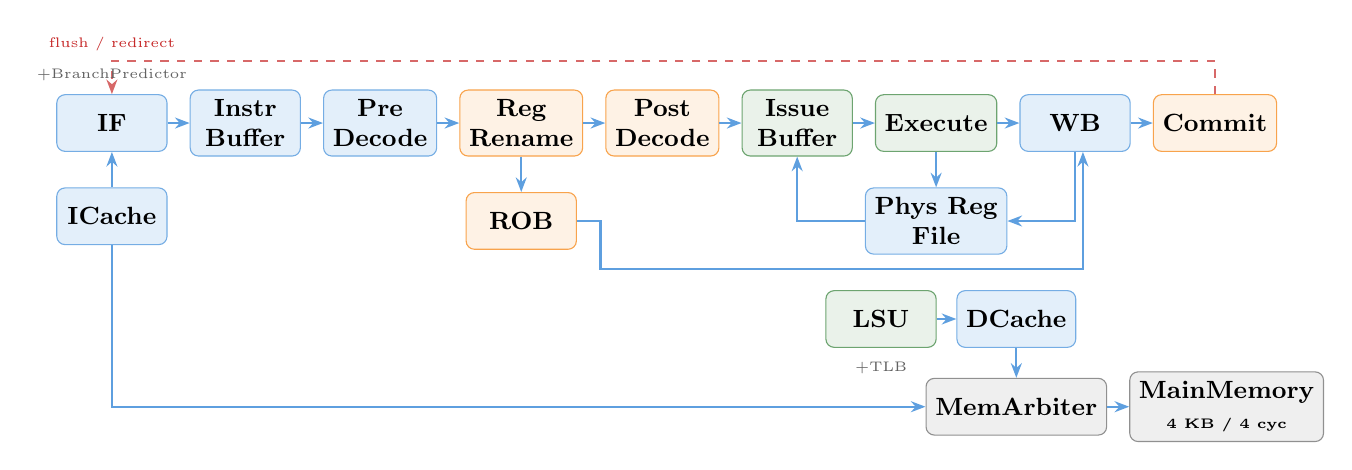
\begin{tikzpicture}[node distance=0.38cm and 0.28cm]
    %% 主流水线（顶行）
    \node[plbox]  (IF)   {IF};
    \node[plbox,  right=of IF]   (IB)   {Instr\\Buffer};
    \node[plbox,  right=of IB]   (PRE)  {Pre\\Decode};
    \node[plobox, right=of PRE]  (RN)   {Reg\\Rename};
    \node[plobox, right=of RN]   (POST) {Post\\Decode};
    \node[plgbox, right=of POST] (RS)   {Issue\\Buffer};
    \node[plgbox, right=of RS]   (EX)   {Execute};
    \node[plbox,  right=of EX]   (WB)   {WB};
    \node[plobox, right=of WB]   (CMT)  {Commit};

    %% 主流水线箭头
    \draw[plarr] (IF)  -- (IB);
    \draw[plarr] (IB)  -- (PRE);
    \draw[plarr] (PRE) -- (RN);
    \draw[plarr] (RN)  -- (POST);
    \draw[plarr] (POST)-- (RS);
    \draw[plarr] (RS)  -- (EX);
    \draw[plarr] (EX)  -- (WB);
    \draw[plarr] (WB)  -- (CMT);

    %% ROB（RN 正下方）
    \node[plobox, below=0.45cm of RN] (ROB) {ROB};
    \draw[plarr] (RN.south)  -- (ROB.north);

    %% PRF（EX 下方）
    \node[plbox, below=0.45cm of EX] (PRF) {Phys Reg\\File};
    \coordinate (RobWBBend) at ($(PRF.south)+(0,-0.18cm)$);
    \draw[plarr] (ROB.east) -- ++(0.3,0) |- (RobWBBend) -| ($(WB.south)+(0.1cm,0)$);
    \draw[plarr] (WB.south) |- (PRF.east);
    \draw[plarr] (PRF.west) -| (RS.south);

    %% ICache（IF 下方）
    \node[plbox, below=0.45cm of IF] (IC) {ICache};
    \draw[plarr] (IC.north) -- (IF.south);

    %% LSU / DCache
    \node[plgbox, below=0.45cm of PRF,xshift=-0.7cm] (LSU) {LSU};
    \node[plbox,  right=0.25cm of LSU]                (DC)  {DCache};
    \draw[plarr] (EX.south)  -- (PRF.north);
    \draw[plarr] (LSU.east)  -- (DC.west);

    %% MemArbiter / MainMemory
    \node[plgrbox, below=0.38cm of DC]               (ARB) {MemArbiter};
    \node[plgrbox, right=0.28cm of ARB]               (MEM) {MainMemory\\{\tiny 4 KB / 4 cyc}};
    \draw[plarr] (IC.south)  |- (ARB.west);
    \draw[plarr] (DC.south)  -- (ARB.north);
    \draw[plarr] (ARB.east)  -- (MEM.west);

    %% Flush 回路
    \draw[plrarr] (CMT.north) -- ++(0,0.42)
      -| node[above,font=\tiny,color=AccentRed]{flush / redirect}
         (IF.north);

    %% 注释
    \node[font=\tiny,color=MidGray,above=0.04cm of IF]  {+BranchPredictor};
    \node[font=\tiny,color=MidGray,below=0.05cm of LSU] {+TLB};
  \end{tikzpicture}}%
  \end{center}

  \vspace{-0.1cm}
  \begin{columns}
    \begin{column}{0.36\textwidth}
      \footnotesize
      \textcolor{PrimaryBlue}{\rule{1em}{0.55ex}}\ 控制/前端/提交\quad
      \textcolor{AccentOrange}{\rule{1em}{0.55ex}}\ 重命名/ROB
    \end{column}
    \begin{column}{0.60\textwidth}
      \footnotesize
      \textcolor{AccentGreen}{\rule{1em}{0.55ex}}\ 发射/执行/访存\quad
      \textcolor{AccentRed!80}{- -}\ flush/redirect（全局广播）
    \end{column}
  \end{columns}
\end{frame}

\begin{frame}[shrink=10]{关键设计参数}
  \begin{columns}[T]
    \begin{column}{0.48\textwidth}
      \small\renewcommand{\arraystretch}{1.22}
      \begin{tabular}{ll}
        \toprule
        \textbf{参数} & \textbf{值} \\
        \midrule
        数据/地址位宽    & 32 位 \\
        超标量宽度       & 2-wide（取指/发射/提交）\\
        ROB 容量         & 32 项，2 位 generation tag \\
        整数物理寄存器   & 64 个（架构 32 个）\\
        浮点物理寄存器   & 64 个 \\
        保留站深度       & 8 项 \\
        指令缓冲深度     & 8 项 \\
        \bottomrule
      \end{tabular}
    \end{column}
    \begin{column}{0.48\textwidth}
      \small\renewcommand{\arraystretch}{1.22}
      \begin{tabular}{ll}
        \toprule
        \textbf{参数} & \textbf{值} \\
        \midrule
        缓存组数/路数    & 64 组 $\times$ 2 路组相联 \\
        缓存行大小       & 128 位（16 字节）\\
        缓存替换策略     & LRU（1 位 per 组）\\
        主存容量         & 4 KB（256 行 $\times$ 16 B）\\
        主存延迟         & 4 周期（固定）\\
        分支预测 GHR     & 8 位全局历史 \\
        PHT / BTB        & 1024 项 PHT，BTB + RAS(8) \\
        \bottomrule
      \end{tabular}
    \end{column}
  \end{columns}
  \vspace{0.3cm}
  \begin{exampleblock}{Generation Tag 防旧写回污染}
    \footnotesize
    每槽 2 位代号，分配时递增；写回时核验\\
    \quad\code{\{rob\_idx, rob\_gen\}}\\
    匹配才接受，防旧写回污染重用槽位。
  \end{exampleblock}
\end{frame}

%% ============================================================
\section{取指前端与分支预测}
%% ============================================================

\begin{frame}{取指前端}{IF + InstructionBuffer + BranchPredictor}
  \begin{columns}[T]
    \begin{column}{0.52\textwidth}
      \begin{block}{IF 模块工作流程}
        \small
        \begin{enumerate}
          \item 向 ICache 发起请求，获取 128 位缓存行（含 4 条指令）
          \item 从缓存行中提取当前 PC 对齐的 \hl{2 条指令}
          \item 调用 BranchPredictor：预测跳转方向 + 目标 PC
          \item 将指令 + PC + 预测信息推入 InstructionBuffer
          \item 次周期 PC $\leftarrow$ 预测目标（推测执行）
        \end{enumerate}
      \end{block}
      \vspace{0.2cm}
      \begin{alertblock}{InstructionBuffer 作用}
        \small 深度 8 的 FIFO，解耦取指（依赖 ICache 延迟）与解码
        （依赖 rename 空闲资源），避免取指停顿直接传播到后端。
      \end{alertblock}
    \end{column}
    \begin{column}{0.44\textwidth}
      \begin{block}{三级分支预测器}
        \small
        \textbf{Gshare PHT}（主预测方向）
        \begin{itemize}
          \item 8 位全局历史寄存器 GHR
          \item $\mathrm{idx} = \mathrm{PC}[9:2] \oplus \mathrm{GHR}$
          \item 1024 项 2-bit 饱和计数器
        \end{itemize}
        \vspace{0.1cm}
        \textbf{BTB}（分支目标缓冲）
        \begin{itemize}
          \item 直接映射，缓存分支目标 PC
          \item 与 PHT 同步查询，取指时立即使用
        \end{itemize}
        \vspace{0.1cm}
        \textbf{RAS}（返回地址栈，深度 8）
        \begin{itemize}
          \item CALL（JAL x1,…）时 push 返回地址
          \item RET（JALR x0,ra,0）时 pop 目标
        \end{itemize}
      \end{block}
    \end{column}
  \end{columns}
\end{frame}

%% ============================================================
\section{寄存器重命名与 ROB}
%% ============================================================

\begin{frame}{寄存器重命名}{消除 WAW/WAR 伪相关，支持乱序执行}
  \begin{columns}[T]
    \begin{column}{0.50\textwidth}
      \begin{block}{核心数据结构}
        \small
        \begin{itemize}
          \item \textbf{映射表（Map Table）}\\
                \code{int\_map[0:31]}：逻辑寄存器 $\to$ 物理寄存器
          \item \textbf{空闲列表（Free List）}\\
                环形队列，管理 p32\textasciitilde p63 共 32 个空闲物理寄存器
          \item \textbf{记分牌（Scoreboard）}\\
                \code{int\_preg\_ready[0:63]}：物理寄存器是否已有有效数据
          \item \textbf{检查点数组（Checkpoint）}\\
                每次 rename\_fire 时快照映射表 + 空闲列表，\\
                flush 时\hl{一周期完成回滚}，无需重放指令
        \end{itemize}
      \end{block}
    \end{column}
    \begin{column}{0.46\textwidth}
      \begin{block}{双指令重命名的批内相关处理}
        \small
        \textbf{批内 RAW（inst1 读 inst0 的写目标）}

        inst1 的源寄存器标签直接使用 inst0 刚分配的\\
        \code{new\_preg}，不查映射表

        \vspace{0.2cm}
        \textbf{批内 WAW（两条指令写同一逻辑寄存器）}

        inst1 的 \code{old\_preg} 取 inst0 的 \code{new\_preg}，\\
        而非映射表中的原始值

        \vspace{0.2cm}
        \textbf{重命名发生阻塞的条件}

        空闲整数/浮点物理寄存器不足，\\
        或 ROB 剩余槽 $< 1$（或 $<2$）时阻塞
      \end{block}
    \end{column}
  \end{columns}
\end{frame}

\begin{frame}{重排序缓冲（ROB）}{顺序提交、精确异常、分支错误恢复}
  \begin{columns}[T]
    \begin{column}{0.50\textwidth}
      \begin{block}{ROB 条目结构（32 项循环队列）}
        \small\renewcommand{\arraystretch}{1.15}
        \begin{tabular}{ll}
          \toprule
          \textbf{字段} & \textbf{说明} \\
          \midrule
          \code{entry\_valid}    & 槽是否被占用 \\
          \code{entry\_ready}    & 执行完毕，可提交 \\
          \code{entry\_pc}       & 指令 PC \\
          \code{entry\_arch\_rd} & 目的架构寄存器 \\
          \code{entry\_new\_preg}& 新分配物理寄存器 \\
          \code{entry\_old\_preg}& 被替换的旧物理寄存器 \\
          \code{entry\_value}    & 执行结果（WB 写入）\\
          \code{entry\_exception}& 是否发生异常 \\
          \code{entry\_gen}      & 2 位代号（防旧写回污染）\\
          \bottomrule
        \end{tabular}
      \end{block}
    \end{column}
    \begin{column}{0.46\textwidth}
      \begin{block}{三种关键操作}
        \small
        \textbf{提交（Commit，2 条/周期）}
        \begin{itemize}
          \item head 条目 valid 且 ready $\Rightarrow$ 提交
          \item 释放 \code{old\_preg} 至空闲列表
          \item 第一条异常时第二条不提交
        \end{itemize}
        \vspace{0.1cm}
        \textbf{写回（3 个 WB 端口）}
        \begin{itemize}
          \item wb0/wb1：INT/Branch/FP/System
          \item wb2：LSU 访存结果
          \item 核验 \code{\{rob\_idx, rob\_gen\}} 防污染
        \end{itemize}
        \vspace{0.1cm}
        \textbf{Flush}
        \begin{itemize}
          \item 分支错误：tail 回退到 \code{flush\_rob\_idx+1}
          \item 精确异常：清空所有条目，跳 TRAP\_VECTOR
        \end{itemize}
      \end{block}
    \end{column}
  \end{columns}
\end{frame}

%% ============================================================
\section{乱序发射与执行}
%% ============================================================

\begin{frame}[shrink=15]{保留站与乱序发射}
  \begin{columns}[T]
    \begin{column}{0.48\textwidth}
      \begin{block}{RS 结构与 CDB 唤醒}
        \small 保留站的深度为 8，全部FU共享一个保留站。

        \small 每个 RS 槽存储一条指令的全部执行信息：
        \begin{itemize}
          \item \textbf{操作数状态}：\code{rs\_ready}（就绪位）、\\
                \code{rs\_tag}（物理寄存器号）、\code{rs\_val}（数值）
          \item \textbf{年龄计数}：\code{rs\_age}\\
                （全局计数器快照，越小越老）
          \item \textbf{CDB 广播唤醒}：WB 结果广播到所有 RS 槽，\\
                匹配 tag 的槽立即获得数值，下周期标记就绪
        \end{itemize}
      \end{block}
      \vspace{0.15cm}
      \begin{alertblock}{发射选择策略}
        \small 每类功能单元独立仲裁：从本类\hl{所有就绪}指令中
        选出\hl{年龄最小}（最老）的发射，保证前进性，避免饥饿。
      \end{alertblock}
    \end{column}
    \begin{column}{0.50\textwidth}
      \begin{block}{功能单元一览}
        \footnotesize\renewcommand{\arraystretch}{1.0}
        \scalebox{0.82}{%
        \begin{tabular}{lp{5.0cm}}
          \toprule
          \textbf{功能单元} & \textbf{说明} \\
          \midrule
          IntALU $\times$ 2    & ADD/SUB/AND/OR/SLL/SLT... \\
          IntMul $\times$ 2  & 单周期乘法 \\
          IntDivider $\times$ 1& 32 周期恢复式除法器（共享）\\
          Branch $\times$ 2    & BEQ/BNE/JAL/JALR + 重定向 \\
          System $\times$ 2    & CSR 读改写（CSRRW/RS/RC）\\
          fpu $\times$ 2 & 浮点（FADD/FSUB/FMUL...）\\
          LSU $\times$ 1       & Load/Store（单 outstanding）\\
          \bottomrule
        \end{tabular}}
      \end{block}
      \vspace{0.15cm}
      \begin{exampleblock}{乱序完成顺序提交}
        \small 各 FU 完成时间不同，后入队指令可能先写回；
        ROB 严格按程序顺序检查 head 是否 ready 后才提交，
        保证精确异常和体系结构一致性。
      \end{exampleblock}
    \end{column}
  \end{columns}
\end{frame}

\begin{frame}{一条指令的完整执行流程}{以 \texttt{ADD x3, x1, x2} 为例}
  \begin{center}
  \begin{tikzpicture}[x=1cm,y=1cm]
    %% ── 第一行：IF → PreDecode → RegRename → PostDecode ──────
    \node[jstep] (s1) at (0,   0) {IF};
    \node[jstep] (s2) at (3.0, 0) {Pre\\Decode};
    \node[jstep] (s3) at (6.0, 0) {Reg\\Rename};
    \node[jstep] (s4) at (9.0, 0) {Post\\Decode};

    \draw[plarr] (s1) -- (s2);
    \draw[plarr] (s2) -- (s3);
    \draw[plarr] (s3) -- (s4);

    %% 第一行描述（下方）
    \node[font=\scriptsize,text=MidGray,
          below=0.1cm of s1,text width=2.5cm,align=center]
      {ICache 取 128b 缓存行，提取 32b 指令字};
    \node[font=\scriptsize,text=MidGray,
          below=0.1cm of s2,text width=2.6cm,align=center]
      {识别 rs1=x1, rs2=x2\\rd=x3, fu=INT};
    \node[font=\scriptsize,text=MidGray,
          below=0.1cm of s3,text width=2.6cm,align=center]
      {x1→p5, x2→p7\\x3→\textcolor{AccentOrange}{\textbf{p42}}（新），old=p3\\快照检查点};
    \node[font=\scriptsize,text=MidGray,
          below=0.1cm of s4,text width=2.5cm,align=center]
      {生成 ALU\_OP\_ADD\\int\_is\_sub=0};

    %% ── 折返箭头：PostDecode → IssueBuffer ───────────────────
    \draw[plarr] (s4.south) -- ++(0,-1.05)
                             -| node[right,font=\tiny,color=MidGray,
                                     xshift=0.05cm,yshift=0.3cm]{} (1.5,-2.2);

    %% ── 第二行：IssueBuffer → Execute → WB/Commit ────────────
    \node[jstep] (s5) at (3.0,-2.2) {Issue\\Buffer};
    \node[jstep] (s6) at (6.0,-2.2) {IntALU};
    \node[jstep] (s7) at (9.0,-2.2) {WB /\\Commit};

    \draw[plarr] (s5) -- (s6);
    \draw[plarr] (s6) -- (s7);

    %% 折返弯箭头（终止于 s5）
    \draw[plarr] (1.5,-2.2) -- (s5.west);

    %% 第二行描述（下方）
    \node[font=\scriptsize,text=MidGray,
          below=0.1cm of s5,text width=2.6cm,align=center]
      {入 RS，等 p5/p7 就绪，年龄最老时发射};
    \node[font=\scriptsize,text=MidGray,
          below=0.1cm of s6,text width=2.5cm,align=center]
      {计算 p5+p7\\单周期完成};
    \node[font=\scriptsize,text=MidGray,
          below=0.1cm of s7,text width=2.6cm,align=center]
      {写 PRF[p42]\\ROB[n].ready=1\\提交时释放 p3};
  \end{tikzpicture}
  \end{center}
  \vspace{-0.1cm}
  \begin{columns}
    \begin{column}{0.48\textwidth}
      \begin{exampleblock}{\small 精确异常保证}
        \small 执行结果写入 ROB 后，只有 head 到达该条目时才更新架构映射，
        推测执行的中间状态对外不可见。
      \end{exampleblock}
    \end{column}
    \begin{column}{0.48\textwidth}
      \begin{exampleblock}{\small 分支错误恢复}
        \small Branch FU 解析实际方向后，若预测错误则发出
        \code{redirect\_valid}，RegRename 从检查点一周期回滚。
      \end{exampleblock}
    \end{column}
  \end{columns}
\end{frame}

%% ============================================================
\section{存储层次结构}
%% ============================================================

\begin{frame}[shrink=4]{存储层次结构}
  \begin{columns}[T]
    \begin{column}{0.43\textwidth}
      \begin{center}
      \begin{tikzpicture}[node distance=0.35cm]
        \node[mboxG] (CPU) {CPU（LSU / IF）};
        \node[mboxB, below=1cm of CPU,xshift=-1.45cm] (IC)
              {ICache\\{\tiny 2-way，64组，128b行}};
        \node[mboxB, below=1cm of CPU,xshift=+1.45cm] (DC)
              {DCache + TLB\\{\tiny 写透+写分配，LRU}};
        \node[mboxGR, below=2.8cm of CPU] (ARB)
              {MemArbiter\\{\tiny D 侧优先}};
        \node[mboxDK,below=1cm of ARB] (MEM)
              {MainMemory\\{\tiny 4 KB，4 周期延迟}};

        \draw[plarr] (CPU.south) -- (IC.north);
        \draw[plarr] (CPU.south) -- (DC.north);
        \draw[plarr] (IC.south)  -- ([xshift=-0.95cm]ARB.north);
        \draw[plarr] (DC.south)  -- ([xshift=+0.95cm]ARB.north);
        \draw[plarr] (ARB.south) -- (MEM.north);
      \end{tikzpicture}
      \end{center}
    \end{column}
    \begin{column}{0.53\textwidth}
      \begin{block}{ICache / DCache 共同参数}
        \small
        \begin{itemize}
          \item 2 路组相联，64 组（\code{CACHE\_INDEX\_BITS=6}）
          \item 缓存行 128 位（4 条 32 位指令或 4 个数据）
          \item Tag 22 位（$32 - 6 - 4 = 22$）
          \item LRU 替换（每组 1 位记录最近使用路）
          \item ICache：只读，缺失时向主存请求填充
          \item DCache：写透传 + 写分配，缺失时先填充再写
        \end{itemize}
      \end{block}
      \vspace{0.15cm}
      \begin{block}{LSU 访存流程}
        \small
        \begin{enumerate}
          \item 对齐检查：misaligned $\to$ 立即异常
          \item TLB 查询：由于操作系统适配未完成，当前 VA = PA，透传
          \item DCache：命中 $\to$ 1 周期返回；\\
                \phantom{DCache：}缺失 $\to$ stall CPU 等主存填充
        \end{enumerate}
        {\footnotesize\textcolor{MidGray}{当前为单 outstanding 设计（无 LSQ / Store Buffer）}}
      \end{block}
    \end{column}
  \end{columns}
\end{frame}

%% ============================================================
\section{仿真验证}
%% ============================================================

\begin{frame}{两个 Testbench}
  \small
  \begin{columns}[T]
    \begin{column}{0.48\textwidth}
      \begin{block}{\texttt{Top\_tb.v} —— 指令测试框架}
        \small
        \begin{itemize}
          \item 面向\hl{单条指令、短指令序列和小型任务级程序}
          \item testbench 直接向主存\hl{动态写入机器码}，无需外部二进制文件
          \item 用于精细验证 ALU、分支、访存、CSR、双发射等功能点
          \item 通过寄存器值、内存内容和提交 PC 等条件判断 PASS / FAIL
        \end{itemize}
      \end{block}
    \end{column}
    \begin{column}{0.48\textwidth}
      \begin{block}{\texttt{Top\_tb\_bin.v} —— 二进制测试框架}
        \small
        \begin{itemize}
          \item 面向\hl{编译后完整程序}的运行验证
          \item 通过 \code{+BIN=<path>} plusarg 加载 编译器生成的 \code{.bin}
          \item 配合简单的binloader \code{crt0.s} 完成结果回传
          \item 运行 C 代码的编译产物测试，验证真实软件执行流程
        \end{itemize}
      \end{block}
    \end{column}
  \end{columns}
  \vspace{0.15cm}
  \begin{exampleblock}{两类 testbench 的分工}
    \small
    \texttt{Top\_tb.v} 偏向 white-box 的功能点定位与定向构造测试；
    \texttt{Top\_tb\_bin.v} 偏向 black-box 的整程序执行验证。下面先介绍前者的指令测试框架，再介绍后者的二进制加载测试框架。
  \end{exampleblock}
\end{frame}

\begin{frame}[shrink=8]{指令测试框架}
  \begin{columns}[T]
    \begin{column}{0.50\textwidth}
      \begin{block}{Testbench 设计要点}
        \small
        \begin{itemize}
          \item 运行时在主存中\hl{动态写入机器码}
          \item 完成检测：监控 ROB 提交时的 PC $=$ \code{init\_ra}（halt循环）
          \item 超时限制：使用最大周期数与最大提交数兜底，防止无限循环
          \item 调试信息：仅失败时输出每周期调试日志
        \end{itemize}
      \end{block}
      \vspace{0.15cm}
      \begin{block}{6 种测试 Task}
        \small
        \renewcommand{\arraystretch}{1.1}
        \begin{tabular}{ll}
          \code{run\_test}          & 单指令寄存器结果验证 \\
          \code{run\_fp\_test}      & 浮点指令验证 \\
          \code{run\_redirect\_test}& 分支跳转 + 重定向 \\
          \code{run\_dual\_test}    & 双发射同批验证 \\
          \code{run\_store\_task}   & Store + 内存内容检查 \\
          \code{run\_task\_test}    & 完整任务级程序运行 \\
        \end{tabular}
      \end{block}
    \end{column}
    \begin{column}{0.46\textwidth}
      \begin{block}{测试覆盖范围与结果}
        \small\renewcommand{\arraystretch}{1.2}
        \begin{tabular}{lcc}
          \toprule
          \textbf{类别} & \textbf{数量} & \textbf{状态} \\
          \midrule
          整数 ALU              & 22 & PASS \\
          分支 / 跳转           & 12 & PASS \\
          Load / Store          & 10 & PASS \\
          MUL / DIV / REM       & 10 & PASS \\
          CSR 指令              & 7  & PASS \\
          除法边界情况          & 4  & PASS \\
          双发射（2-wide）      & 8  & PASS \\
          分支预测恢复          & 4  & PASS \\
          \midrule
          \textbf{任务级 sum()} & \textbf{1} & \gcheck \textbf{PASS}\\
          \midrule
          \textbf{合计}         & \textbf{78} & \textbf{全部通过} \\
          \bottomrule
        \end{tabular}
      \end{block}
    \end{column}
  \end{columns}
\end{frame}

\begin{frame}[fragile,shrink=6]{指令测试框架 —— 任务级测试}
  \begin{columns}[T]
    \begin{column}{0.50\textwidth}
      \begin{block}{测试程序（C，源代码：https://gcc.godbolt.org/z/3nY96eaYc）}
\begin{lstlisting}[language=C]
// sum(a,b): a + (a+1) + ... + b
// sum(10, 20) = 145
int sum(int a, int b) {
    int i = 0;
    int target = b - a;
    int ret = 0;
    while (i < target) {
        ret += a + i;
        i += 1;
    }
    return ret;
}

int main() {
    int result = sum(10, 20); // -> 145
    // halt loop (j .)
}
\end{lstlisting}
      \end{block}
    \end{column}
    \begin{column}{0.46\textwidth}
      \begin{block}{测试要点}
        \small
        \begin{itemize}
          \item 函数调用：测试JAL/JALR，完整栈帧（push/pop ra, s0）环境
          \item 循环 + 条件分支：测试分支预测与重定向
          \item Load/Store：测试访存
          \item 算术运算：测试数据依赖问题，重命名与ALU

        \end{itemize}
      \end{block}
      \vspace{0.15cm}
      \begin{exampleblock}{验证结果}
        \small
        仿真输出：\code{PASS\_TASK[70] commits=N}

        验证项目：
        \begin{itemize}
          \item \code{a0} 寄存器 $=$ \textcolor{AccentGreen}{\textbf{145}}（期望值）
          \item \code{sp} 恢复到初始值 \code{0x0F00}
          \item 内存地址 \code{0xEE4} 存有 145
        \end{itemize}
      \end{exampleblock}
    \end{column}
  \end{columns}
\end{frame}

\begin{frame}{二进制测试框架}
  \begin{columns}[T]
    \begin{column}{0.52\textwidth}
      \begin{block}{软件测试工具链}
        \footnotesize
        \begin{itemize}
          \item 基础工具链：\code{riscv64-unknown-elf-gcc}，\code{-march=rv32i -mabi=ilp32 -nostdlib -nostartfiles}
          \item \textbf{crt0.s}：初始化 SP、清零 BSS、调用 \code{main()}、写 \code{tohost}
          \item \textbf{link.ld}：规定程序区 \code{0x1000–0x1FD0}；\\
                \code{tohost @0x1FF0}（0=PASS/非零=FAIL）；\code{putchar @0x1FE0}
          \item \textbf{Top\_tb\_bin.v}：通过 \code{+BIN=<path>} plusarg 加载 \code{.bin}文件，监视主存的tohost 写入，
                超时或 FAIL 时打印调试上下文（寄存器/栈/提交记录）
        \end{itemize}
      \end{block}
    \end{column}
    \begin{column}{0.44\textwidth}
      \begin{block}{sw/ 测试结果（7 个用例）}
        \footnotesize\renewcommand{\arraystretch}{1.15}
        \begin{tabular}{ll}
          \toprule
          \textbf{测试用例} & \textbf{状态} \\
          \midrule
          test\_add\_123.c     & PASS \\
          test\_add\_notest2.c & PASS \\
          test\_sub\_simple.c  & PASS \\
          test\_regkeep.c      & PASS \\
          test\_regkeep2.c     & PASS \\
          \midrule
          test\_add.c          & \textcolor{AccentRed}{\bfseries FAIL (code 3)} \\
          test\_add\_noref.c   & \textcolor{AccentRed}{\bfseries FAIL (code 3)} \\
          \bottomrule
        \end{tabular}
      \end{block}
      \vspace{0.08cm}
      \begin{alertblock}{已知 Bug（待修复）}
        疑似特定指令序列触发 rename/checkpoint 边缘情况。
      \end{alertblock}
    \end{column}
  \end{columns}
\end{frame}

%% ============================================================
\section{总结与展望}
%% ============================================================

\begin{frame}{局限性与未来工作}
  \begin{columns}[T]
    \begin{column}{0.48\textwidth}
      \begin{alertblock}{当前已知局限性}
        \small
        \begin{itemize}
          \item \textbf{LSU 单 outstanding}：无 LSQ / Store Buffer，不支持乱序访存和 Load Forwarding
          \item \textbf{主存仅 4 KB}：大型程序无法运行
          \item \textbf{FP 支持不完整}：fma/div/sqrt/cvt 等缺失
          \item \textbf{异常模型简化}：无完整 mepc/mcause 元数据流
          \item \textbf{检查点开销大}：$32 \times 32 \times 2$ 快照数组较占资源
          \item \textbf{sw/ 测试 Bug未解决}：特定调用序列后结果错误（FAIL code 3），根因未知，疑似是 rename/checkpoint 边缘情况
        \end{itemize}
      \end{alertblock}
    \end{column}
    \begin{column}{0.48\textwidth}
      \begin{exampleblock}{改进点}
        \small
        \begin{enumerate}
          \item \textbf{访存子系统升级}：引入 LSQ + Store Buffer，支持乱序 Load/Store 调度与 Load Forwarding
          \item \textbf{FP 完整实现}：接入完整 fma/div/sqrt
          \item \textbf{性能计数器}：添加 stall 原因、预测命中率、Cache miss 率等统计
          \item \textbf{压力测试}：CDB 高并发写回、多重 redirect 的恢复等场景
          \item \textbf{扩展主存}：支持更大程序
        \end{enumerate}
      \end{exampleblock}
    \end{column}
  \end{columns}
\end{frame}

\begin{frame}{总结}
  \vfill
  \begin{center}
    \begin{minipage}{0.78\textwidth}
      \begin{block}{已实现的核心特性}
        \raggedright
        \begin{itemize}
          \item \textbf{2-wide 超标量乱序执行}\\
          \item \textbf{精确异常与分支快速恢复}\\
          \item \textbf{RV32I + M 完整实现，F部分实现}\\
          \item \textbf{两级缓存层次结构}\\
          \item \textbf{Gshare + BTB + RAS 分支预测}\\
        \end{itemize}
      \end{block}
    \end{minipage}
  \end{center}
  \vspace{0.2cm}
  \begin{center}
    \large\textcolor{PrimaryBlue}{\textbf{感谢聆听！欢迎提问。}}
  \end{center}
  \vfill
\end{frame}

%% ─── 附录 ────────────────────────────────────────────────────
\appendix

\begin{frame}[fragile,shrink=6]{附录 A：全局冲刷信号链}{Top.v 控制逻辑}
  \begin{block}{全局冲刷逻辑（Top.v）}
\begin{lstlisting}[language=Verilog]
// Two triggers: misprediction OR precise exception
wire commit_exc   = commit0_exception;
wire global_flush = redirect_valid | commit_exc;
wire flush_target = redirect_valid ? redirect_target
                                   : TRAP_VECTOR;
\end{lstlisting}
  \end{block}
  \vspace{0.2cm}
  \begin{columns}[T]
    \begin{column}{0.48\textwidth}
      \begin{block}{分支预测错误恢复}
        \small
        \begin{enumerate}
          \item Branch FU 解析实际方向与目标
          \item 发出 \code{redirect\_valid + redirect\_target}
          \item ROB 清除该分支之后的年轻条目，tail 回退
          \item RegRename 从对应检查点恢复映射表和空闲列表
          \item IF 重定向到正确 PC，下周期继续取指
        \end{enumerate}
      \end{block}
    \end{column}
    \begin{column}{0.48\textwidth}
      \begin{block}{精确异常处理}
        \small
        \begin{enumerate}
          \item ROB head 提交时检测 \code{commit0\_exception}
          \item 触发全局 flush，清空 ROB 所有条目
          \item RegRename 重置映射表到提交后架构状态
          \item PC 跳转到 \code{TRAP\_VECTOR}（\code{0x0000\_1000}）
        \end{enumerate}
      \end{block}
    \end{column}
  \end{columns}
\end{frame}

\begin{frame}{附录 B：ROB Generation Tag 机制}
  \begin{exampleblock}{为什么需要 Generation Tag？}
    \small
    考虑以下场景：
    \begin{enumerate}
      \item 指令 A 进入 ROB[5]，发射到执行单元（慢操作，如除法）
      \item 发生 flush（分支预测错误），ROB[5] 被清空
      \item 新指令 B 重新分配 ROB[5]（generation 自增）
      \item 指令 A 的写回信号 \code{wb\_rob\_idx=5} 此时才到达
    \end{enumerate}
    \vspace{0.1cm}
    若无保护机制，写回会错误地将 B 的 ROB 条目标记为 ready！
  \end{exampleblock}
  \vspace{0.2cm}
  \begin{block}{Generation Tag 解决方案}
    \small
    \begin{itemize}
      \item 每个 ROB 槽维护 2 位代号 \code{entry\_gen}，每次分配时递增
      \item 写回时携带 \code{wb\_rob\_gen}，ROB 仅当
            \code{entry\_gen[idx] == wb\_rob\_gen} 时才接受写回
      \item flush 后 B 拥有新的 gen 值，A 的旧 gen 不匹配，写回被安全丢弃
    \end{itemize}
  \end{block}
\end{frame}

\end{document}
